\documentclass[11pt]{article}

\usepackage{float}
\usepackage{hyperref}
\usepackage{enumerate}
\usepackage{graphicx}
\usepackage{amsmath}
\usepackage{epstopdf}
\usepackage{minted}
\usepackage{parskip}
\usepackage[toc,page]{appendix}
\usepackage{gensymb}
% formatting
\usepackage{fullpage}
\usepackage{verbatim}
\let\verbatiminput=\verbatimtabinput
\def\verbatimtabsize{4\relax}

\begin{document}
\title{EE 142 Lab 0 Report - Agilent ADS Introduction}

\author{Vighnesh Iyer}
\date{Monday, August 28, 2017}
\maketitle

\section{DC Simulation}
I setup a DC simulation to characterize the Predictive Transistor Model (PTM) BSIM4 MOSFET device. It's nominal supply is $V_{DD} = 0.9V$ and we sweep its $V_{DS}$ and $V_{GS}$ and record the drain current $I_{DS}$ reported by the model.

\subsection{$I_{ds}$ vs $V_{gs}$ and $I_{ds}$ vs $V_{ds}$}
\begin{figure}[H]
	\minipage{0.50\textwidth}
	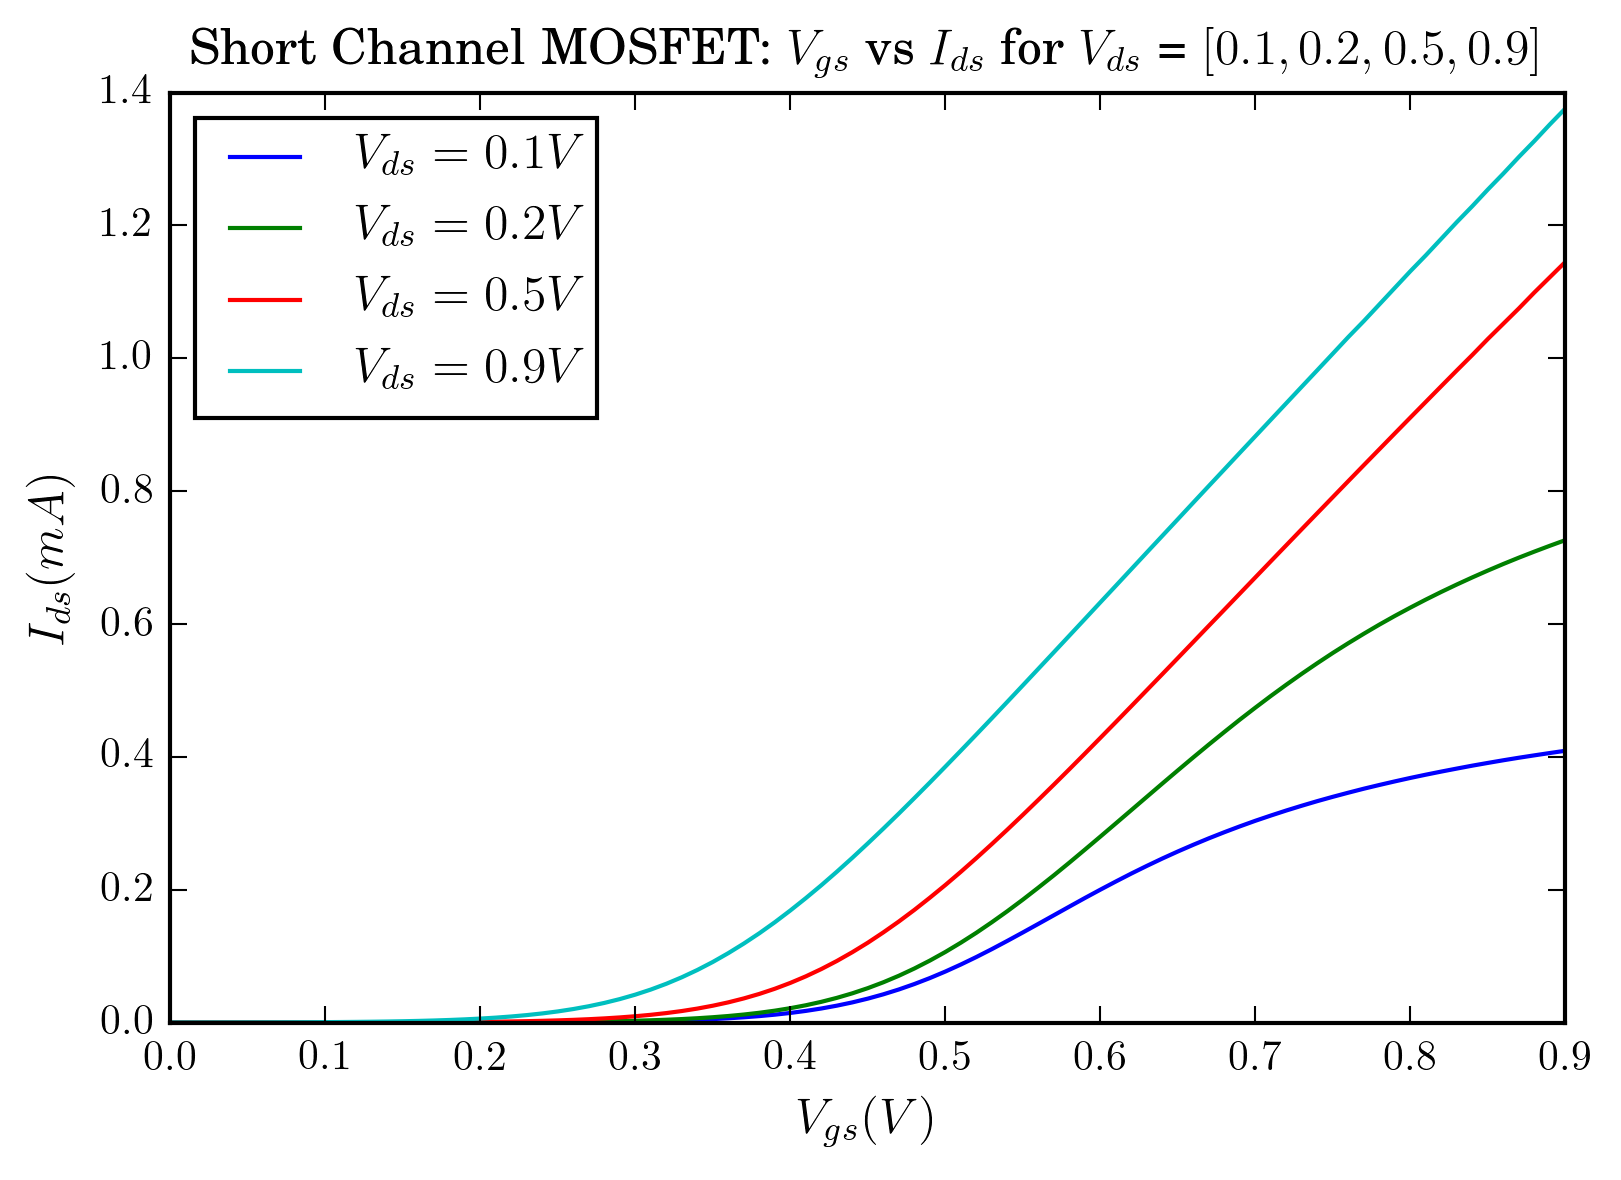
\includegraphics[width=\linewidth]{images/short_channel_vgs_vs_ids.png}
	\endminipage\hfill
	\minipage{0.50\textwidth}
	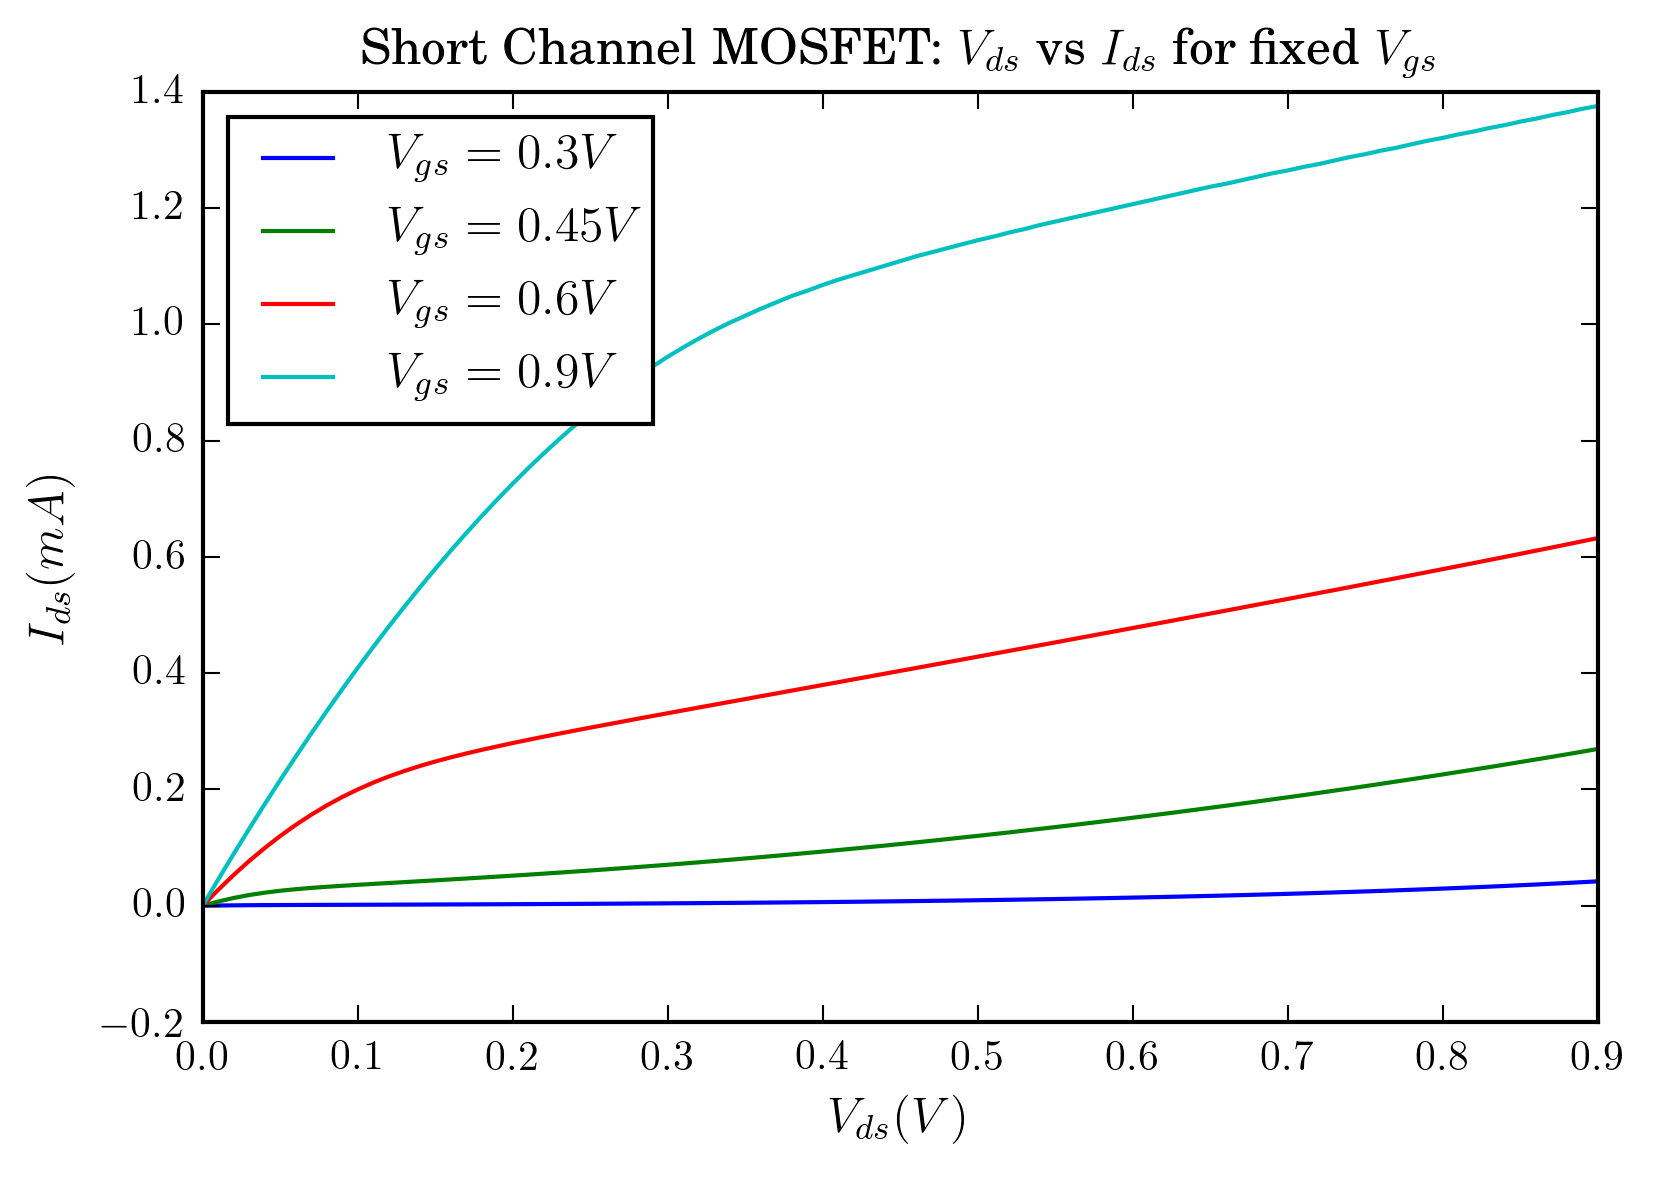
\includegraphics[width=\linewidth]{images/short_channel_vds_vs_ids.png}
	\endminipage
\end{figure}

\subsection{Long-Channel vs. Short-Channel MOSFETs}
I used the built-in/default Level 3 MOSFET model in ADS to represent a typical long-channel MOSFET model. Its I-V curves are plotted below.
\begin{figure}[H]
	\minipage{0.50\textwidth}
	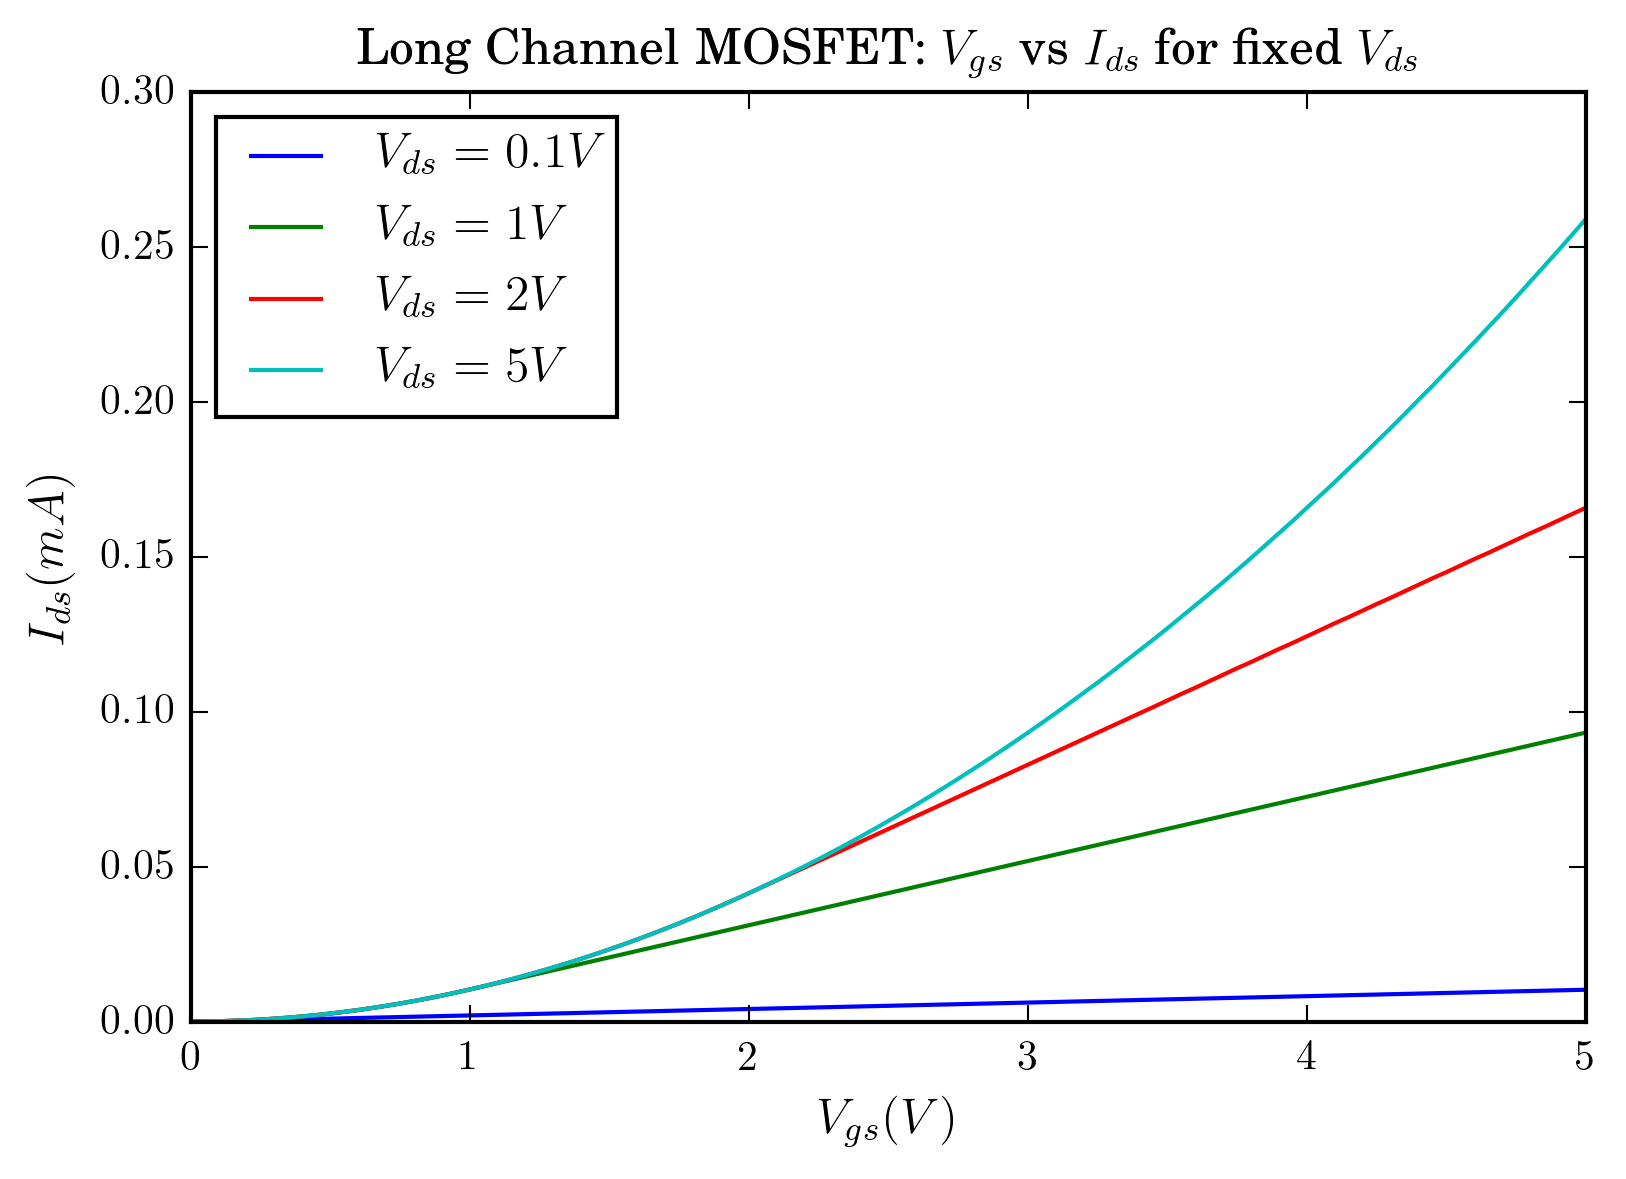
\includegraphics[width=\linewidth]{images/long_channel_vgs_vs_ids.png}
	\endminipage\hfill
	\minipage{0.50\textwidth}
	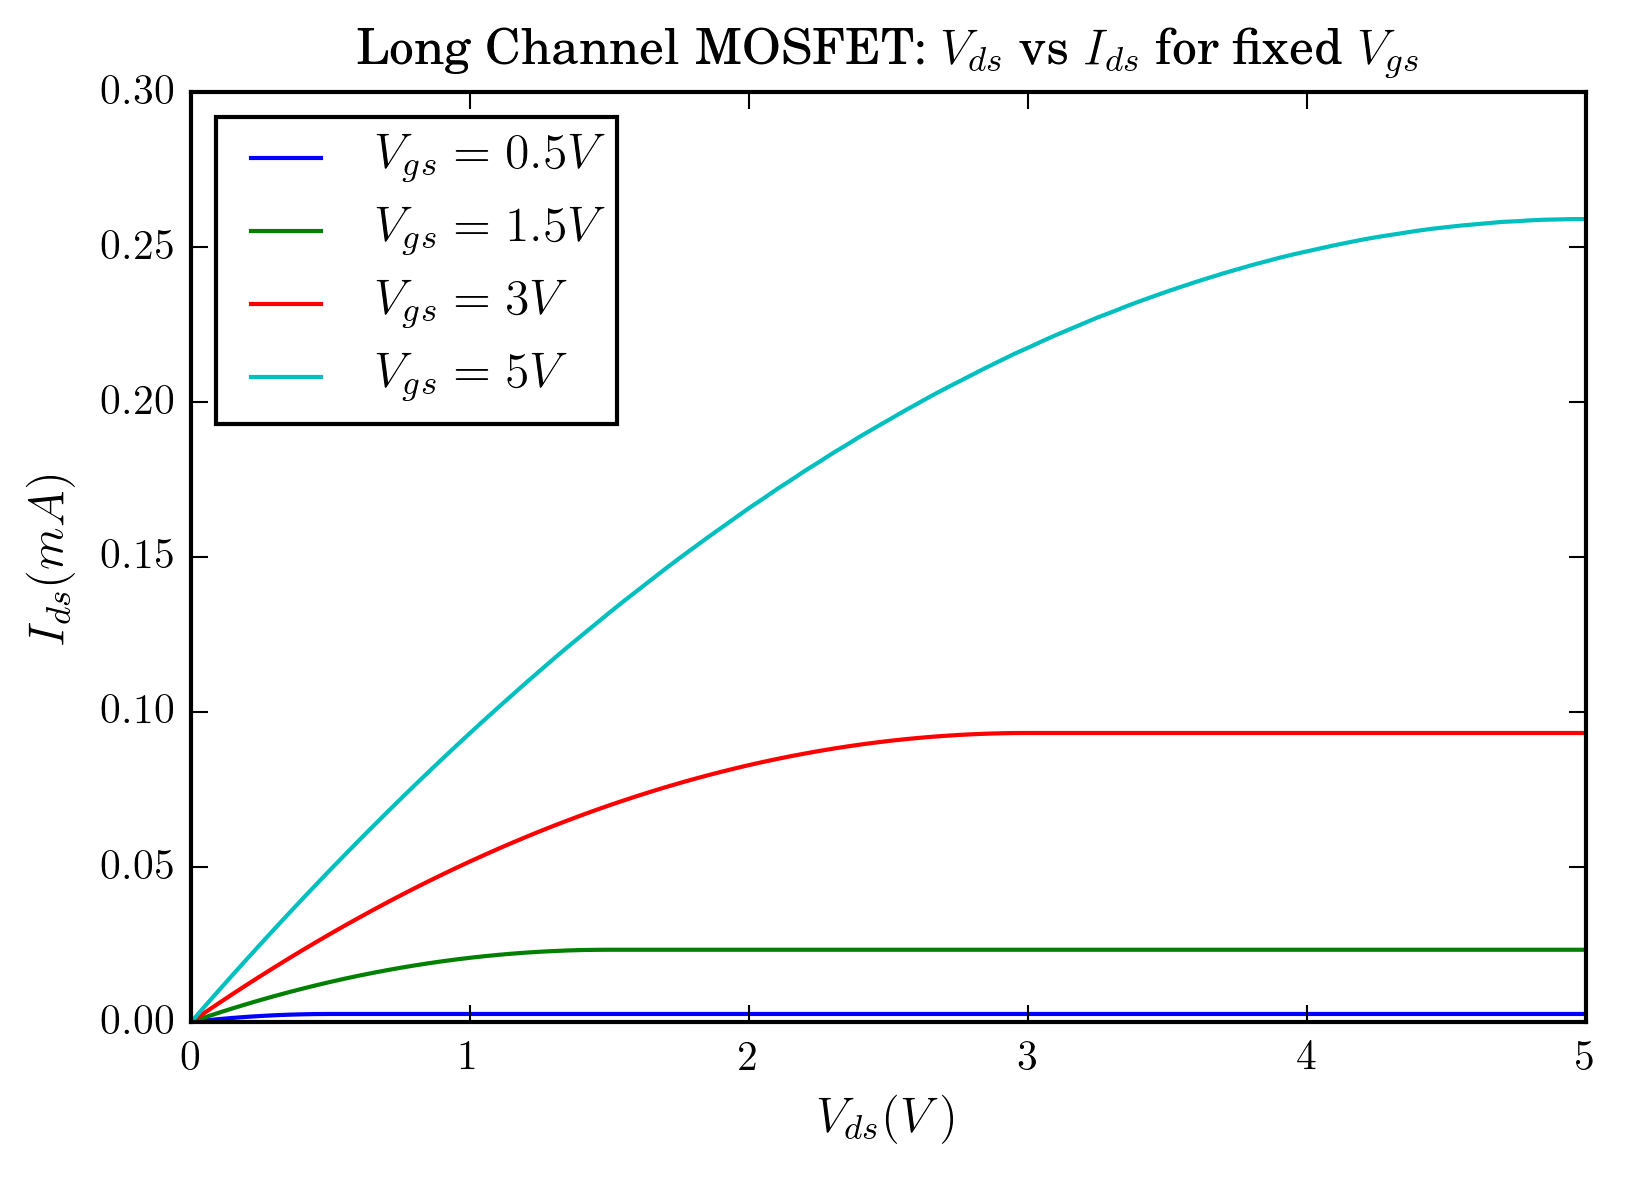
\includegraphics[width=\linewidth]{images/long_channel_vds_vs_ids.png}
	\endminipage
\end{figure}

We can see some major differences in the shape of the curves, which can be explained by various short-channel effects:

\begin{itemize}
	\item DIBL (drain induced barrier lowering)
	\item Channel length modulation (equivalent to BJT early effect)
	\item 
\end{itemize}

\newpage
\appendix
\section{Example} \label{ex}

\end{document}